\documentclass[a4paper,11pt,fleqn]{article}%fleqn pour aligner les equations à gauche
\usepackage{/home/rweye/Nextcloud/Documents/Overleaf/Styles/Cours}

\newcommand{\chnum}{Fiche méthode 1}
\newcommand{\chtitle}{Spectroscopie infrarouge}
\newcommand{\dtype}{TSPE}

\begin{document}
\maketitle

\section{Principe de la spectroscopie infrarouge}
La spectroscopie infrarouge est une technique expérimentale consistant à analyser le rayonnement infrarouge traversant un échantillon. Une partie du rayonnement est absorbée par la substance et cela se traduit par la présence de bandes d'absorption caractéristiques de certaines liaisons.
\begin{figure}[h!]
    \centering
    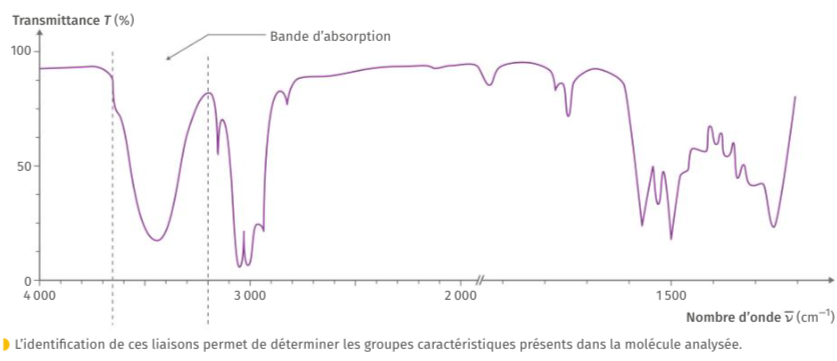
\includegraphics[width =.9\linewidth]{Ressources/TSPE_F1_fig1.png}
\end{figure}

\section{Bandes d'absorption et liaisons}
\begin{tabular}{|>{\centering}m{.15\linewidth}|>{\centering}m{.45\linewidth}|>{\centering \arraybackslash} m{.3\linewidth}|}
    \hline
    \textbf{Liaison} &\textbf{Condition} & \textbf{Nombre d'onde} $\overline{\nu}$ (\unit{\per\centi\meter})\\
    \hline
    \chemfig{O-H} & Sans pont hydrogène & \num{3580} - \num{3650} (bande fine)\\ \cline{2-3}
    & Avec pont hydrogène & \num{3200} - \num{3400} (bande large)\\ \cline{2-3}
    & Si cette liaison  fait partie du groupe caractéristique carbonyle & \num{2500} - \num{3200} (bande large)\\ \cline{2-3}
    \hline
    \chemfig{N-H} & - & \num{3400} - \num{3500}\\
    \hline
    \chemfig{C-H} & - & \num{2800} - \num{3100}\\ \cline{2-3}
    & Si l'atome de carbone est lié par une liaison double avec un atome d'oxygène & \num{2750} - \num{2900}\\ \cline{2-3}
    \hline
    \chemfig{C=O} & Si cette liaison fait partie du groupe carbonyle & \num{1650} - \num{1730}\\ \cline{2-3}
    & Si cette liaison fait partie du groupe carboxyle & \num{1680} - \num{1710}\\ \cline{2-3}
    & Si cette liaison fait partie du groupe caractéristique ester & \num{1700} - \num{1740}\\ \cline{2-3}
    & Si cette liaison fait partie du groupe caractéristique amide & \num{1650}\\
    \hline
    \chemfig{C=C} & Si cette liaison ne fait pas partie d'un sycle aromatique & \num{1640} - \num{1680}\\ \cline{2-3}
    & Si cette liaison fait partie d'un sycle aromatique & \num{1500} - \num{1580}\\
    \hline 
\end{tabular}
\end{document}